\documentclass[pdf]{beamer}
\usetheme{Copenhagen}
\usepackage{pgfgantt}
% Need to use LuaLatex to compile
\usepackage{emoji}
\usepackage{booktabs}
\usepackage{tikz}
\usepackage{fontawesome}
\usepackage{amsmath}
\usepackage{natbib}
\usepackage[most]{tcolorbox}
\tcbuselibrary{skins}
\usetikzlibrary{angles,calc,intersections,quotes,arrows.meta,positioning}
\setemojifont{Apple Color Emoji}
\setbeamercovered{transparent}
\beamertemplatenavigationsymbolsempty
\setbeamertemplate{footline}[text line]{%
\parbox{\linewidth}{\vspace*{-8pt}\hfill\hfill\insertframenumber\,/\,\inserttotalframenumber}}

\title{``$2^{\text{nd}}$'' Year PhD Seminar Presentation}

\author[Ananth Mahadevan]{Ananth Mahadevan}
\date{\today}
\usepackage{xspace}
\newcommand*{\error}{\ensuremath{\accDis}\xspace}
\newcommand*{\accuracy}{\ensuremath{\acctest}\xspace}

% training 
\newcommand*{\D}{\ensuremath{\mathcal{D}}\xspace}
\newcommand*{\sample}{\ensuremath{\mathbf{x}}\xspace}
\newcommand*{\dimensions}{\ensuremath{d}\xspace}
\newcommand*{\labels}{\ensuremath{\mathbf{y}}\xspace}

\newcommand*{\Dtrain}{\ensuremath{\D_{\text{init} }}\xspace}
\newcommand*{\Dm}{\ensuremath{\mathcal{D}_{\nremovals}}\xspace}
\newcommand*{\Dprime}{\ensuremath{\D\setminus\Dm}\xspace}
\newcommand*{\Dtest}{\ensuremath{\mathcal{D}_{\text{test}}}\xspace}
\newcommand*{\nremovals}{\ensuremath{m}\xspace}
\newcommand*{\ntrain}{\ensuremath{n_{\text{init}}}\xspace}
\newcommand*{\ntest}{\ensuremath{n}_{\text{test}}\xspace}
\newcommand*{\obj}{\ensuremath{L}\xspace}

%
\newcommand*{\UM}{\ensuremath{u}\xspace}
\newcommand*{\ml}{ML\xspace}
\newcommand*{\sgd}{SGD\xspace}
\newcommand*{\w}{\ensuremath{\mathbf{w}}\xspace}
\newcommand*{\wopt}{\ensuremath{\w^{opt}}\xspace}
\newcommand*{\worig}{\ensuremath{\mathbf{w}^{*}}\xspace}
\newcommand*{\employed}{\ensuremath{e}\xspace}
\newcommand*{\wEmployed}{\ensuremath{\w}\xspace}
\newcommand*{\wunlearned}{\ensuremath{\w^\UM}\xspace}
\newcommand*{\wprime}{\ensuremath{\mathbf{w}^{\prime}}\xspace}
% 

\newcommand*{\efficiencyParameter}{\ensuremath{\tau}\xspace}
\newcommand*{\QoA}{\ensuremath{\efficiencyParameter}\xspace}
\newcommand*{\noiseParamter}{\ensuremath{\sigma}\xspace}
\newcommand*{\unlrbatchsize}{\ensuremath{\nremovals^{\prime}}\xspace}
% Guo et al. 
\newcommand*{\noisyobj}{\ensuremath{\obj_{\sigma}}\xspace}
\newcommand*{\infl}{\textsc{Influence}\xspace}
\newcommand*{\guo}{\textsc{guo}\xspace}

% Golatkar et al.
\newcommand*{\fisher}{\textsc{Fisher}\xspace}
\newcommand*{\fMatrix}{\ensuremath{F}\xspace}
\newcommand*{\gol}{\textsc{gol}\xspace}

% Wu et al. 
\newcommand*{\wu}{\textsc{wu}\xspace}
\newcommand*{\deltagrad}{\textsc{DeltaGrad}\xspace}
\newcommand*{\iw}{\ensuremath{\w}\xspace}
\newcommand*{\dgapprox}{\textsc{DGApprox}\xspace}

% Distribution Experiment
\newcommand*{\classprob}{p_{\text{class}}\xspace}
\newcommand*{\infoprob}{p_{\text{info}}\xspace}

% Datasets

\newcommand*{\bmnist}{\ensuremath{\text{\sc mnist}^{\text{b}}}\xspace}
\newcommand*{\mnist}{\text{\sc mnist}\xspace}
\newcommand*{\covtype}{\text{\sc covtype}\xspace}
\newcommand*{\higgs}{\text{\sc higgs}\xspace}
\newcommand*{\cifar}{\text{\sc cifar2}\xspace}
\newcommand*{\eps}{\text{\sc epsilon}\xspace}
\newcommand*{\T}{\top}
\newcommand*{\x}{\mathbf{x}\space}
\newcommand*{\noiseb}{\ensuremath{\mathbf{b}}\xspace}

% metrics
\newcommand{\smape}{\ensuremath{\text{\tt SMAPE}}\xspace}
\newcommand{\sape}{\ensuremath{\text{\tt SAPE}}\xspace}
\newcommand{\acctest}{\ensuremath{\text{\tt Acc}_{\text{test}}}\xspace}
\newcommand{\accremoved}{\ensuremath{\text{\tt Acc}_{\text{del}}}\xspace}
\newcommand*{\accErr}{\texttt{AccErr}\xspace}
\newcommand*{\accDrop}{\accErr}
\newcommand*{\relEff}{\accDrop}
\newcommand*{\accDis}{\texttt{AccDis}\xspace}

% sampling types 

\newcommand{\unirand}{\text{{\tt uniform-random}}\xspace}
\newcommand{\targrand}{\text{{\tt targeted-random}}\xspace}
\newcommand{\uniinfo}{\text{{\tt uniform-informed}}\xspace}
\newcommand{\targinfo}{\text{{\tt targeted-informed}}\xspace}

% When to retrain
\newcommand*{\winit}{\ensuremath{\worig_{\text{init}}}\xspace}
\newcommand*{\accdropinit}{\ensuremath{\accDrop_{\text{init}}}\xspace}
\newcommand*{\acctestinit}{\ensuremath{\acctest^{\text{init}}}\xspace}
\newcommand*{\slope}{\ensuremath{c}\xspace}
\newcommand*{\disPred}{\ensuremath{\overline{\error}}\xspace}
\newcommand*{\estErr}{\ensuremath{EstErr}\xspace}
\newcommand*{\estDis}{\ensuremath{EstDis}\xspace}
\newcommand*{\thresh}{\ensuremath{\kappa}\xspace}

%
\newcommand*{\repo}{\url{https://version.helsinki.fi/mahadeva/unlearning-experiments}}

\newcommand*{\good}{\ensuremath{\uparrow}}
\newcommand*{\better}{\ensuremath{\uparrow\uparrow}}
\newcommand*{\best}{\ensuremath{\uparrow\uparrow\uparrow}}
\newcommand{\revision}[1]{\textcolor{blue}{{#1}}}

\newcommand*{\inc}{\ensuremath{\textcolor{green!80!black}\uparrow}}
\newcommand*{\dec}{\ensuremath{\textcolor{red!80!black}\downarrow}}







\usepackage{xspace}
\usepackage{amsmath}
\usepackage{amssymb}
\usepackage{subcaption}



\newcommand{\norm}[1]{\|#1\|}
\newcommand{\inner}[2]{\langle #1, #2 \rangle}
\newcommand{\round}[1]{\left(#1\right)}
\newcommand{\braces}[1]{\left\{#1\right\}}
\newcommand{\squares}[1]{\left[#1\right]}
\newcommand{\product}[1]{\left\langle#1\right\rangle}

% \newcommand*{\ml}{ML}

\newcommand*{\decision}{\ensuremath{\mathcal{R}}\xspace}
% \newcommand*{\QDM}{\ensuremath{\text{\sc QDM}}\xspace}
\newcommand*{\QDMq}{\ensuremath{\psi}\xspace}
\newcommand*{\QDM}{\ensuremath{\Psi}\xspace}
% \newcommand*{\QDMdiff}{\ensuremath{\QDM_{\text{diff}}}\xspace}
\newcommand*{\QDMdiff}{\ensuremath{\overline{\Psi}}\xspace}
\newcommand*{\simfn}{\ensuremath{\text{sim}}\xspace}
\newcommand*{\loss}{\ensuremath{\ell}\xspace}
\newcommand*{\tprime}{\ensuremath{t^{\prime}}\xspace}
\newcommand*{\feat}{\ensuremath{d}\xspace}
\newcommand*{\q}{\ensuremath{q}\xspace}
% \newcommand*{\x}{\ensuremath{x}\xspace}
\newcommand*{\y}{\ensuremath{y}\xspace}
\newcommand*{\X}{\ensuremath{\mathbf{X}}\xspace}
\newcommand*{\Y}{\ensuremath{\mathbf{y}}\xspace}
\newcommand*{\Yset}{\ensuremath{\mathcal{Y}}\xspace}
\newcommand*{\Xset}{\ensuremath{\mathcal{X}}\xspace}
\newcommand*{\ttime}{\ensuremath{t}\xspace}
\newcommand*{\data}{\ensuremath{D}\xspace}
\newcommand*{\model}{\ensuremath{M}\xspace}
\newcommand*{\query}{\ensuremath{Q}\xspace}
\newcommand*{\Dtprime}{\ensuremath{\data_{\tprime}}\xspace}
\newcommand*{\Mtprime}{\ensuremath{\model_{\tprime}}\xspace}
\newcommand*{\Qtprime}{\ensuremath{\query_{\tprime}}\xspace}
\newcommand*{\Dt}{\ensuremath{\data_{t}}\xspace}
\newcommand*{\Mt}{\ensuremath{\model_{t}}\xspace}
\newcommand*{\Qt}{\ensuremath{\query_{t}}\xspace}
\newcommand*{\dataBatch}{\ensuremath{B_\data}\xspace}
\newcommand*{\queryBatch}{\ensuremath{B_\query}\xspace}
% \newcommand*{\T}{\ensuremath{T}\xspace}
\newcommand*{\offline}{\text{offline}\xspace}
\newcommand*{\online}{\text{online}\xspace}
\newcommand*{\Toffline}{\ensuremath{\T_{\offline}}\xspace}
\newcommand*{\Tonline}{\ensuremath{\T_{\online}}\xspace}
\newcommand*{\Tstart}{\ensuremath{\T_{\text{start}}}\xspace}
\newcommand*{\Tend}{\ensuremath{\T_{\text{end}}}\xspace}
\newcommand*{\Cost}{\ensuremath{C}\xspace}
\newcommand*{\totalcost}{\ensuremath{c}\xspace}
\newcommand*{\cost}[1]{\ensuremath{\text{cost}\round{#1}}\xspace}
\newcommand*{\dpcost}[2][]{%
    \ifx\\#1\\%
        \ensuremath{v\round{#2}}\xspace%
        \else%
        \ensuremath{v^{#1}\round{#2}}\xspace%
    \fi%
}
\newcommand*{\prev}{\ensuremath{p}\xspace}
\newcommand*{\dptable}{\ensuremath{V}\xspace}
\newcommand*{\costmatrix}{\Cost}
\newcommand*{\costentry}[1]{\ensuremath{c_{#1}}\xspace}
\newcommand*{\strategy}{\ensuremath{S}\xspace}
\newcommand*{\partialstrategy}{\ensuremath{\bar{\strategy}}\xspace}
\newcommand*{\partialstrategyopt}{\ensuremath{\round{\partialstrategy}^{*}}\xspace}

\newcommand*{\oracleretrains}{\ensuremath{O}\xspace}
\newcommand*{\retraincost}{\ensuremath{\kappa}\xspace}

\newcommand*{\retrain}{\texttt{Retrain}\xspace}
\newcommand*{\keep}{\texttt{Keep}\xspace}


%algorithms

\newcommand*{\oracle}{\textsc{Oracle}\xspace}
\newcommand*{\neverretrain}{\textsc{NR}\xspace}
\newcommand*{\algo}{\textsc{Cara}\xspace}
\newcommand*{\cara}{\algo}
\newcommand*{\algoparams}{\ensuremath{\theta}\xspace}
\newcommand*{\algoparamsopt}{\ensuremath{\algoparams^{*}}\xspace}

\newcommand*{\markov}{\textsc{Markov}\xspace}
\newcommand*{\algoMarkov}{\textsc{\algo-M}\xspace}
\newcommand*{\algoThresh}{\textsc{\algo-T}\xspace}
% \newcommand*{\thresh}{\ensuremath{\tau}\xspace}
\newcommand*{\threshopt}{\ensuremath{\thresh^{*}}\xspace}
\newcommand*{\cumthresh}{\ensuremath{\tau_\text{cum}}\xspace}
\newcommand*{\cumthreshopt}{\ensuremath{\cumthresh^{*}}\xspace}

\newcommand*{\algoCummThresh}{\textsc{\algo-CT}\xspace}
\newcommand*{\algoPeriod}{\textsc{\algo-P}\xspace}
\newcommand*{\period}{\ensuremath{\phi}\xspace}
\newcommand*{\periodopt}{\ensuremath{\period^{*}}\xspace}
\newcommand*{\offset}{\ensuremath{a}\xspace}
\newcommand*{\offsetopt}{\ensuremath{\offset^{*}}\xspace}


%baselines
\newcommand*{\adwin}{\textsc{ADWIN}\xspace}
\newcommand*{\ddm}{\textsc{DDM}\xspace}

%metrics 
\newcommand*{\scpe}{\texttt{SCPE}\xspace}
%datasets
\newcommand*{\covcon}{\textsc{CovCon}\xspace}
\newcommand*{\covconData}{\textsc{\covcon-D}\xspace}
\newcommand*{\covconStatic}{\textsc{\covcon-S}\xspace}
\newcommand*{\Circle}{\textsc{Circle}\xspace}
\newcommand*{\Circles}{\Circle}
\newcommand*{\circles}{\Circle}
\newcommand*{\circlesData}{\textsc{\Circle-D}\xspace}
\newcommand*{\circlesStatic}{\textsc{\Circle-S}\xspace}
\newcommand*{\gauss}{\textsc{Gauss}\xspace}
\newcommand*{\gaussData}{\textsc{\gauss-D}\xspace}
\newcommand*{\gaussStatic}{\textsc{\gauss-S}\xspace}
\newcommand*{\elec}{\textsc{Electricity}\xspace}
\newcommand*{\covertype}{\textsc{Covertype}\xspace}
% \newcommand*{\covtype}{\textsc{Covtype}\xspace}
\newcommand*{\airlines}{\textsc{Airlines}\xspace}
\newcommand*{\fixedretraincost}{\ensuremath{46}}


\begin{document}
\begin{frame}
    \titlepage
\end{frame}

\begin{frame}
    \frametitle{Quick Recap}
    \begin{itemize}
        \item \textbf{Masters:} Aalto University
        \item \textbf{Started:} Aug 2020 (contract) and Jan 2021 (study right) 
        \item \textbf{Supervisor:} Michael Mathioudakis
        \item \textbf{Research Group:} Algorithmic Data Science (ADS)
    \end{itemize}

    

\end{frame}

\begin{frame}[fragile]
    \frametitle{PhD Progress}
    \begin{ganttchart}[
        % hgrid,
        % vgrid,
        bar/.append style={fill=gray!50},
        time slot format=isodate-yearmonth,
        time slot unit=month,
        x unit=1.5mm,
        y unit chart=7mm,
        % y unit=1mm,
        progress label text={\pgfmathprintnumber[precision=0, verbatim]{#1}\%},
        % progress=today,
        today=2024-03,
        bar height=.5,
        group peaks width=1,
        group peaks height=0.4,
        rejected/.style={milestone/.append style={fill=red}},
        published/.style={milestone/.append style={fill=green}},
        review/.style={milestone/.append style={fill=yellow}},
        futurepublished/.style={milestone/.append style={fill=gray!50}},
        % bar top shift=.5
      ]{2020-01}{2024-12}
    \gantttitlecalendar{year} \\
      \ganttgroup[progress=today]{PhD}{2020-08}{2024-12}\\
      \ganttbar{Paper I}{2021-01}{2021-06} % Unlearning 
      \ganttmilestone[rejected]{}{2021-07} % VLDB-2022
      \ganttmilestone[rejected]{}{2022-02} % ECML_PKDD
      \ganttmilestone[published]{}{2022-04}\\ % MDPI-MAKE
      \ganttbar{Paper II}{2022-01}{2022-02} % JANE
      \ganttmilestone[rejected]{}{2022-03} % ANS extension 2022
      \ganttmilestone[published]{}{2022-06}\\
      \ganttbar{Paper III}{2020-08}{2020-09} % Sketching
      \ganttbar{}{2021-06}{2021-09} % Sketching
      \ganttbar{}{2022-03}{2022-05} % Sketching
      \ganttmilestone[published]{}{2022-09}\\ % CIKM 2022
      \ganttbar{Paper IV}{2022-05}{2023-02} % Reception Reader
      \ganttmilestone[published]{}{2023-04}\\ % JOHD 2023
      \ganttbar{Paper V}{2022-11}{2023-04} % Mandeville
      \ganttmilestone[published]{}{2023-12}\\ % JOHD 2023
      \ganttbar{Paper VI}{2021-11}{2022-12} % UpdateML
      \ganttmilestone[rejected]{}{2023-03} % ICML 2023
      \ganttmilestone[rejected]{}{2023-08} % EuroSys 2024
      \ganttmilestone[review]{}{2024-02}\\ % KBS 2024
      \ganttbar{Paper VII}{2023-06}{2024-02} % TextReuse Pipeline
      \ganttmilestone[futurepublished]{}{2024-04}\\ % KBS 2024

    \end{ganttchart}    

\end{frame}


\begin{frame}
    \frametitle{Papers}
    \begin{table}
        \centering
        \begin{tabular}{cccc}
            \toprule
            Number & One Word Title & Venue & Include in Thesis? \\
            \midrule
            I & Unlearning & MAKE 2022  & \emoji{check-mark-button}  \\
            II & JANE & Entropy 2022   &\emoji{check-mark-button} \\
            III & Sketching& CIKM 2022 & \emoji{man-shrugging-medium-skin-tone}\\
            IV & ReceptionReader& JOHD 2023 &  \emoji{man-shrugging-medium-skin-tone} \\
            V & Mandeville & DES 2023 & \emoji{man-shrugging-medium-skin-tone}\\
            VI & Retraining & KBS 2024 &  \emoji{check-mark-button} \\
            VII & TextReuse & VLDB 2024 & \emoji{check-mark-button} \\

            
        \end{tabular}
    \end{table}
\end{frame}


\begin{frame}
    \frametitle{Research Projects}
    % \begin{block}{\centering Broad Research Interests}
    %     \begin{center}
    %         Scalable Pipelines for Machine Learning and Data Science
    %     \end{center}
    % \end{block}

    Multiple Projects:
    \begin{enumerate}
        \item Maintaining ML models
        \begin{itemize}
            \item Paper I: Unlearning 
            \item Paper VI: Retraining
        \end{itemize}
        \item Analyzing Historical Documents 
        \begin{itemize}
            \item Paper IV: ReceptionReader
            \item Paper V: Mandeville
            \item Paper VII: TextReuse
        \end{itemize}
        \item Scaling and Evaluating Algorithms
        \begin{itemize}
            \item Paper II: JANE
            \item Paper III: Sketching 
            \item Paper VIII    ?: Diverse Sampling 
        \end{itemize}
    \end{enumerate}

\end{frame}


\begin{frame}
    \frametitle{Maintaining ML models}

    \begin{block}{\centering Research Question}
        \centering
        How to update a trained ML model when the data changes?
    \end{block}

    \begin{enumerate}
        \item Machine Unlearning 
        \begin{itemize}
            \item Training data is deleted/removed
            \item Update model parameters to forget information
            \item \citet{mahadevan2022certifiable}
        \end{itemize}
        \item Cost-Aware Retraining
        \begin{itemize}
            \item Streams drift over time
            \item Data and Queries are present
            \item Retraining consumes resources
            \item When is it worth retraining?
            \item \citet{mahadevan2023costeffective}
        \end{itemize}
    \end{enumerate}
\end{frame}


\begin{frame}
    \frametitle{Machine Unlearning }
    \scalebox{0.5}{
    \begin{tikzpicture}
        \newcommand\file[2]{%
    \begin{scope}[xshift=#1cm,yshift=#2cm]
      \draw[gray,thick] (0,0) -- (0,1.5) -- (0.7,1.5) -- (0.7,1.1) -- (1,1.1) -- (1,0) -- cycle;
      \draw[gray,thick] (0.7,1.5) -- (1,1.1);
      \foreach \y in {0.2,0.3,...,1.1}{
         \draw[thick] (0.2,\y) -- (0.8,\y);
         }
      \foreach \y in {1.1,1.2,...,1.4}{
         \draw[thick] (0.2,\y) -- (0.65,\y);
         }
        %  \draw[thick] (0.2,0.8) -- (0.6,0.8);
        %  \draw[thick] (0.2,1) -- (0.6,1);
    \end{scope}
}

% https://tex.stackexchange.com/questions/126161/how-can-i-draw-a-tikz-element-multiple-times-against-a-shaded-background
% \pgfkeys{/tikz/.cd,
%    at/.initial={(0,0)},
%    at/.get=\coordpos,
%    at/.store in=\coordpos,   
%    my tree/.code={
%     \draw[gray] \coordpos -- +(0,1.2) -- +(0.7,1.2) -- +(0.7,0.8) -- +(1,0.8) -- +(1,0) -- cycle;
%     \draw[gray] +(0.7,1.2) -- +(1,0.8);
%     \foreach \y in {0.2,0.4,0.6}{
%         \draw (0.2,\y) -- (0.8,\y);
%         \draw (0.2,0.8) -- (0.6,0.8);
%         \draw (0.2,1) -- (0.6,1);
%     }
%    }
% }
\begin{tikzpicture}
    \tikzset{
      piece/.style 2 args={red,draw,thick,rectangle,anchor=south west,minimum width=#1,minimum height=#2},
      defrag piece/.style 2 args={blue,draw,thick,rectangle,anchor=south west,minimum width=#1,minimum height=#2},
      source piece/.style 2 args={orange,draw,very thick,rectangle,anchor=south west,minimum width=#1,minimum height=#2},
      destination piece/.style 2 args={green!50!black,draw,very thick,rectangle,anchor=south west,minimum width=#1,minimum height=#2},
      reuse/.style={red,-,very thick},
      defrag reuse/.style={blue,-,very thick},
      reception/.style={black,-{Latex[scale=1]},very thick},
    %   cluster/.style={violet,-,very thick}
    cluster/.style={violet,-,very thick,rounded corners=10pt,rectangle},
    }
    \begin{scope}[local bounding box=scope1]
    % \draw [help lines] (0,-2) grid (4,4);
    \file{0}{0}
    \node at (0.5,1.65) {A};
    \node[piece={0.8cm}{0.4cm}] at (0.1,0.1) (tr11) {};
    \node[piece={0.54cm}{0.4cm}] at (0.1,1.1) (tr12) {};
    \file{1.5}{1.5}
    \node at (2,3.15) {B};
    \node[piece={0.8cm}{0.4cm}] at (1.55,1.55) (tr21) {};
    \node[piece={0.78cm}{0.5cm}] at (1.64,1.63) (tr22) {};
    \file{3}{0}
    \node at (3.5,1.65) {C};
    \node[piece={0.54cm}{0.4cm}] at (3.1,0.95) (tr31) {};
    \node[piece={0.8cm}{0.4cm}] at (3.1,0.1) (tr32) {};
    \file{1.5}{-1.5}
    \node at (2,0.15) {D};
    \node[piece={0.8cm}{0.4cm}] at (1.55,-1.45) (tr41) {};
    \node[piece={0.78cm}{0.5cm}] at (1.63,-1.36) (tr42) {};
    \draw[reuse] (tr12.east) -- (tr21.west);
    \draw[reuse] (tr11.east) -- (tr41.west);
    \draw[reuse] (tr42.east) -- (tr32.west);
    \draw[reuse] (tr22.east) -- (tr31.west);
    % \node at (2,-1.68) {};
    % \matrix [below left] at (current bounding box.north east) {
    % \node [piece={0.5cm}{0.1cm},label=right:Piece] {};\\
    % \node[reuse,inner sep=0,minimum width=4mm,draw,anchor= south west,label=right:Text Reuse] at ++(1mm,0) {};\\
    % };
    \end{scope}
    \uncover<2->{
    \begin{scope}[local bounding box=scope2,shift={(scope1.base east)},xshift=3cm]
    % \draw [help lines] (0,-2) grid (4,4);
    \file{0}{0}
    \node at (0.5,1.65) {A};
    \node[defrag piece={0.8cm}{0.4cm}] at (0.1,0.1) (tr11) {};
    \node[defrag piece={0.54cm}{0.4cm}] at (0.1,1.1) (tr12) {};
    \file{1.5}{1.5}
    \node at (2,3.15) {B};
    \node[defrag piece={0.8cm}{0.54cm}] at (1.58,1.6) (tr21) {};
    \file{3}{0}
    \node at (3.5,1.65) {C};
    \node[defrag piece={0.54cm}{0.4cm}] at (3.1,0.95) (tr31) {};
    \node[defrag piece={0.8cm}{0.4cm}] at (3.1,0.1) (tr32) {};
    \file{1.5}{-1.5}
    \node at (2,0.15) {D};
    \node[defrag piece={0.8cm}{0.54cm}] at (1.6,-1.4) (tr41) {};
    \draw[defrag reuse] (tr12.east) -- (tr21.west);
    \draw[defrag reuse] (tr11.east) -- (tr41.west);
    \draw[defrag reuse] (tr41.east) -- (tr32.west);
    \draw[defrag reuse] (tr21.east) -- (tr31.west);
    
    % \draw[cluster] plot [smooth cycle] coordinates{(0.1,1) (3.8,0.95) (3.5,2) (2,2.25) (0.6,2) };
    % \draw[cluster] plot [smooth cycle] coordinates{(0.0,0.6)  (4,0.6) (3.5,-1) (2,-1.75) (0.55,-1)};
    \uncover<3->{
    \draw[cluster] (-0.1,0.9) rectangle (4,2.3) ;
    \draw[cluster] (-0.1,0.6) rectangle (4,-1.5) ;
    }
    \end{scope}
    \draw [->,black,very thick] ($(scope1.east)!0.1!(scope2.west)$) -- ($(scope1.east)!0.9!(scope2.west)$) node[midway,above,align=center]{Defragment} node[midway,below] {\only<3->{\& Cluster}};
    }
    \uncover<4->{
    \begin{scope}[local bounding box=scope3,shift={(scope2.base east)},xshift=3cm]
      % \draw [help lines] (0,-2) grid (4,4);
      \file{0}{0}
      \node at (0.5,1.65) {A};
      \node[source piece={0.8cm}{0.4cm}] at (0.1,0.1) (tr11) {};
      \node[alt=<-4>{defrag piece={0.54cm}{0.4cm}}{destination piece={0.54cm}{0.4cm}}] at (0.1,1.1) (tr12) {};
      \file{1.5}{1.5}
      \node at (2,3.15) {B};
      \node[source piece={0.8cm}{0.54cm}] at (1.58,1.6) (tr21) {};
      \file{3}{0}
      \node at (3.5,1.65) {C};
      \node[alt=<-4>{defrag piece={0.54cm}{0.4cm}}{destination piece={0.54cm}{0.4cm}}] at (3.1,0.95) (tr31) {};
      \node[alt=<-4>{defrag piece={0.8cm}{0.4cm}}{destination piece={0.8cm}{0.4cm}}] at (3.1,0.1) (tr32) {};
      \file{1.5}{-1.5}
      \node at (2,0.15) {D};
      \node[alt=<-4>{defrag piece={0.8cm}{0.54cm}}{destination piece={0.8cm}{0.54cm}}] at (1.6,-1.4) (tr41) {};
      \uncover<6->{
      \draw[reception] (tr11.east) -- (tr41.west);
      \draw[reception] (tr11.east) -- (tr32.west);

      \draw[reception] (tr21.west) -- (tr12.east);
      \draw[reception] (tr21.east) -- (tr31.west);
      }
    %   \draw[cluster] plot [smooth cycle] coordinates{(0.1,1) (3.8,0.95) (3.5,2) (2,2.25) (0.6,2) };
    %   \draw[cluster] plot [smooth cycle] coordinates{(0.0,0.6)  (4,0.6) (3.5,-1) (2,-1.75) (0.55,-1)};
    \draw[cluster] (-0.1,0.9) rectangle (4,2.3) ;
    \draw[cluster] (-0.1,0.6) rectangle (4,-1.5) ;
      \end{scope}
      
      
      \draw [->,black,very thick] ($(scope2.east)!0.1!(scope3.west)$) -- ($(scope2.east)!0.9!(scope3.west)$) node[midway,above]{Identify Source}  node[midway,below] {\only<5->{\& Destinations}};
      
    }
    \matrix [draw,matrix anchor = south,yshift=5mm] at (current bounding box.north)
    % ($(scope1.north west)!0.5!(scope3.north east)$) 
    {
    \node [piece={0.5cm}{0.1cm},label=right:Piece] {}; & 
      \node [defrag piece={0.5cm}{0.1cm},label=right:Defrag Piece] {}; &
      \node [source piece={0.5cm}{0.1cm},label=right:Src Piece] {}; &
      \node[draw,cluster,anchor=south west,minimum width=0.5cm,minimum height=0.1cm,rounded corners=2pt,rectangle,label=right:Cluster] {};\\
    %   \node [destination piece={0.5cm}{0.1cm},label=right:Destination Piece] {}; &\\
      \node[reuse,inner sep=0,minimum width=4mm,draw,anchor=south west,label=right:Reuse] at ++(0,1mm) {}; &
      \node[defrag reuse,inner sep=0,minimum width=4mm,draw,anchor= south west,label=right:Defrag Reuse] at ++(0,1mm) {}; &
      \node [destination piece={0.5cm}{0.1cm},label=right:Dest Piece] {}; &
      \draw[reception] (0,1mm) -- (5mm,1mm) node[inner sep =0,minimum size =0,right,anchor=west] {Reception};
      \node [inner sep=0,label=right:Doc,anchor=south west] at (2.2cm,-0.5mm){\faFileTextO};&
    \\
    };
\end{tikzpicture}
      \end{tikzpicture}
    }

    \begin{block}{Unlearning}
        Task of updating a ML model after partial deletion of training data
    \end{block}
    Qualities of an approximate unlearning method:
  \begin{itemize}
    \item \textbf{Certifiability}: How similar are \wunlearned and \worig?
    \item \textbf{Effectiveness}: How well does \wunlearned perform?
    \item \textbf{Efficiency}: How much time to produce \wunlearned?
  \end{itemize}

\end{frame}

\begin{frame}
    \frametitle{Experimental Setup}
    \begin{center}
        \begin{tabular}{cc}
          \toprule
          Item & Values  \\
          \midrule
          Parameters & Noise (\noiseParamter) \& Efficiency (\efficiencyParameter)  \\
          Metrics & \accDis, \accErr \& Speedup(\texttimes) \\
          Methods & \textcolor{blue!80!black}{\infl}, \textcolor{orange!90!black}{\fisher} \& \textcolor{green!60!black}{\deltagrad}\\
          \bottomrule
        \end{tabular}
      \end{center}
      \begin{center}
        \begin{tabular}{cc}
          \toprule
          Metric & Quality \\
          \midrule
          \accDis\inc & Certifiability\dec\\
          \accErr\inc & Effectiveness\dec\\
          \bottomrule
        \end{tabular}
    \end{center}
        \begin{center}
            \begin{tabular}{cc}
              \toprule
              Parameter & Effect\\
              \midrule
              $\efficiencyParameter\inc$ & $\text{Efficiency}\inc\text{ Certifiability}\dec\text{ Effectiveness}\dec$\\
              $\noiseParamter\inc$ & $\text{Certifiability}\inc\text{ Effectiveness}\dec$\\ 
              \bottomrule
            \end{tabular}
        \end{center}
\end{frame}

\begin{frame}[fragile]
    \frametitle{Cost-Aware Retraining Algorithms}
    \tcbset{
          beamer alerted/.style={colframe=blue!50!gray},
        }
    \begin{tcbraster}[raster columns=2, raster left skip=-0.9cm,raster right skip=-0.9cm,raster before skip=0mm]
        \begin{tcolorbox}[nobeforeafter, title=Cost Matrix,,left=0mm,top=0mm,boxsep=0.5mm,alert=<1>]
            \begin{center}
            \begin{equation*}
                \small
                C[t^\prime,t]
            \end{equation*}
            \begin{align*}
                \small
                = \begin{cases}
                    \text{\footnotesize Staleness Cost} \quad& \text{\small if } t^\prime< t\\
                    \text{\footnotesize Retraining Cost} \quad& \text{\small if } t^\prime=t\\
                    \infty \quad&  \text{\small otherwise} 
                \end{cases}
            \end{align*}
        \end{center}
        \begin{center}
            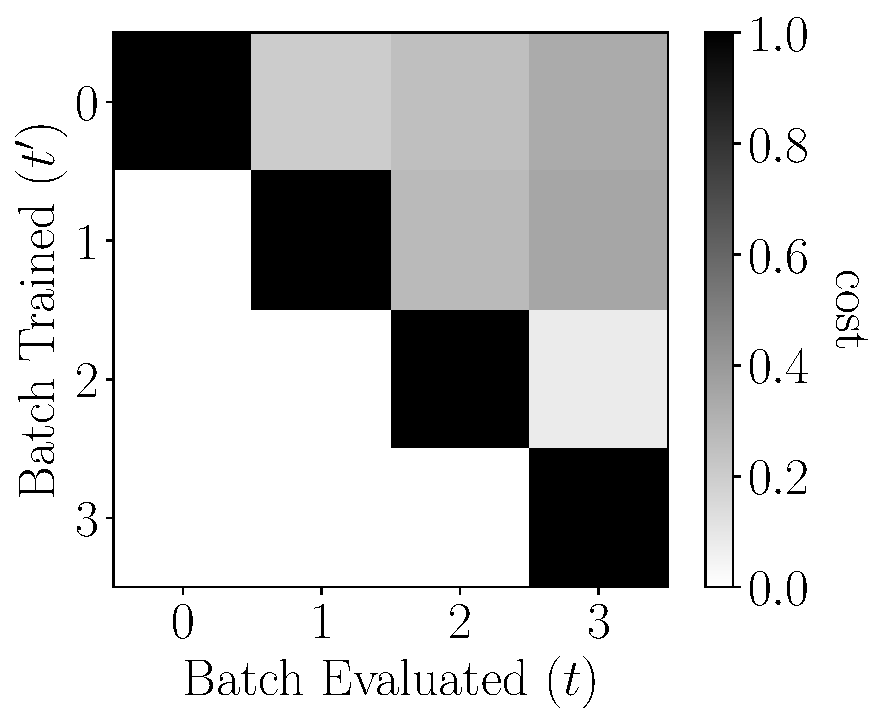
\includegraphics[width=.78\textwidth]{figs/cost_matrix.pdf}
                    \end{center}
        \end{tcolorbox}
        \begin{tcolorbox}[nobeforeafter, title=Strategy,boxsep=0.5mm,left=0mm,alert=<2>]
            \setlength{\leftmargini}{0.4cm}
            \begin{itemize}
            \item Strategy is a set of decisions
            \item \retrain or \keep
            \item Cost of decisions is strategy cost
            \item Aim is to minimize strategy cost
        \end{itemize}
        $$S = \braces{\keep,\keep,\retrain,\retrain}$$
        \begin{center}
            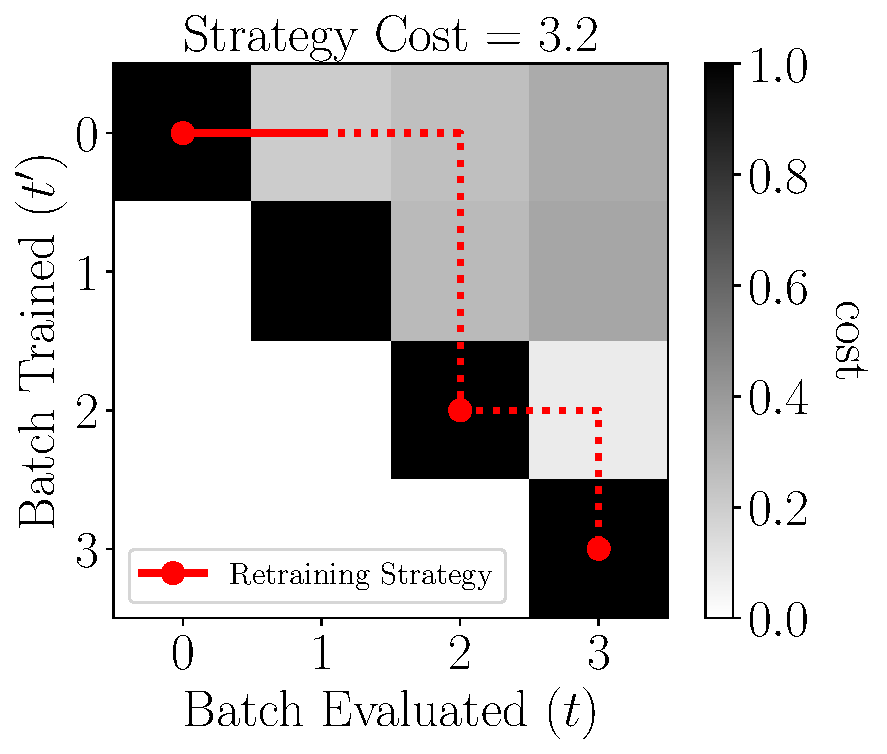
\includegraphics[width=.78\textwidth]{figs/strategy.pdf}
            \end{center}
            \end{tcolorbox}
    \end{tcbraster}
\end{frame}


\begin{frame}
    \frametitle{Retraining Cost \retraincost}
    \begin{itemize}
        \item Trade-off parameter between resources \& performance
        \item Low \retraincost
        \begin{itemize}
          \item Performance is important
          \item Frequent \retrain decisions to minimize staleness cost 
        \end{itemize}
        \item High \retraincost
        \begin{itemize}
          \item Resources are important
          \item \retrain decisions when large enough drops in performance
        \end{itemize}
      \end{itemize}
        \begin{minipage}{0.5\textwidth}
          \begin{center}
              {\footnotesize Low \retraincost}\\[1mm]
              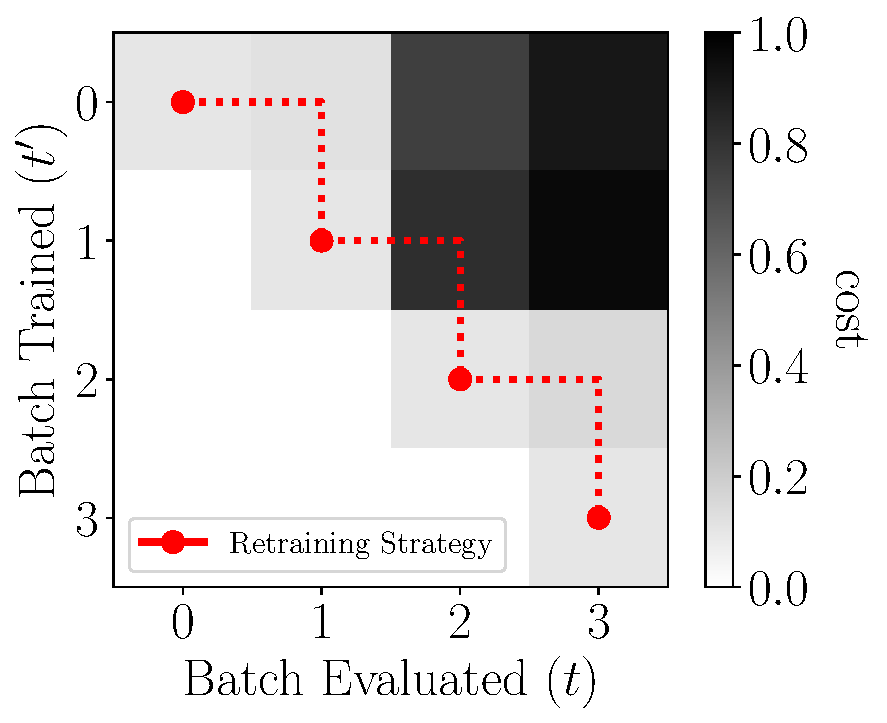
\includegraphics[width=\textwidth]{figs/low_retrain_cost.pdf}
          \end{center}
        \end{minipage}%
        \begin{minipage}{0.5\textwidth}
          \begin{center}
              {\footnotesize High \retraincost}\\[1mm]
              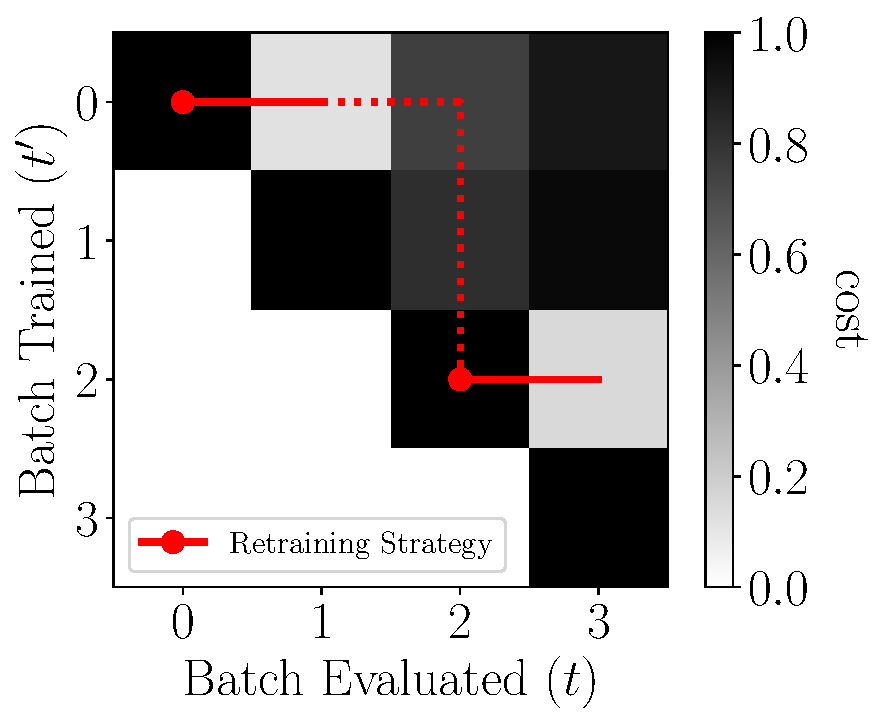
\includegraphics[width=\textwidth]{figs/high_retrain_cost.pdf}
          \end{center}
        \end{minipage}%
    

\end{frame}


\begin{frame}
    \frametitle{Staleness Cost}
    \begin{itemize}
        \item {\textcolor{green!50!black}{Query-aware}} performance cost of old model \Mtprime at batch \ttime
        \item Scenario 1: Low staleness ~~~ Scenario 2: High staleness
      \end{itemize}
      \begin{minipage}{0.5\textwidth}
          \begin{center}
            %   {\footnotesize Scenario 1}\\[1mm]
              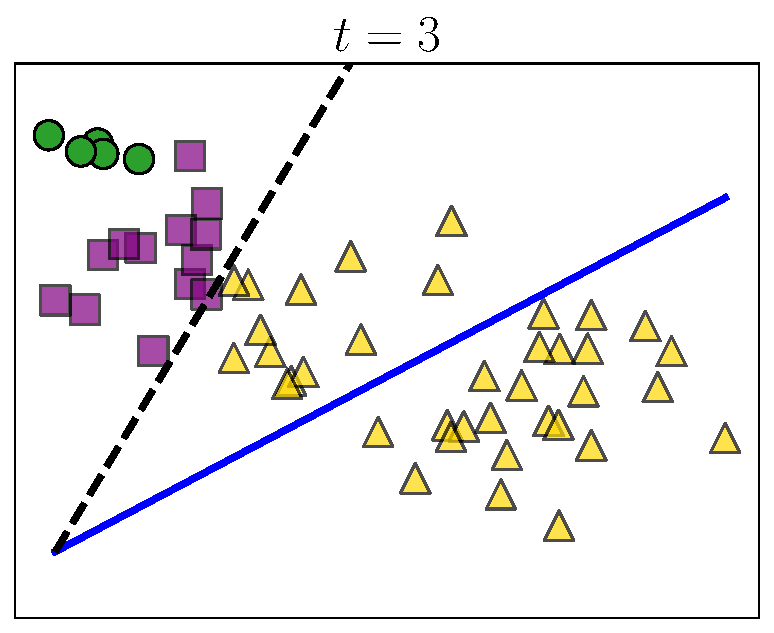
\includegraphics[width=0.7\textwidth]{figs/far_queries_illustration.pdf}\\[1mm]
              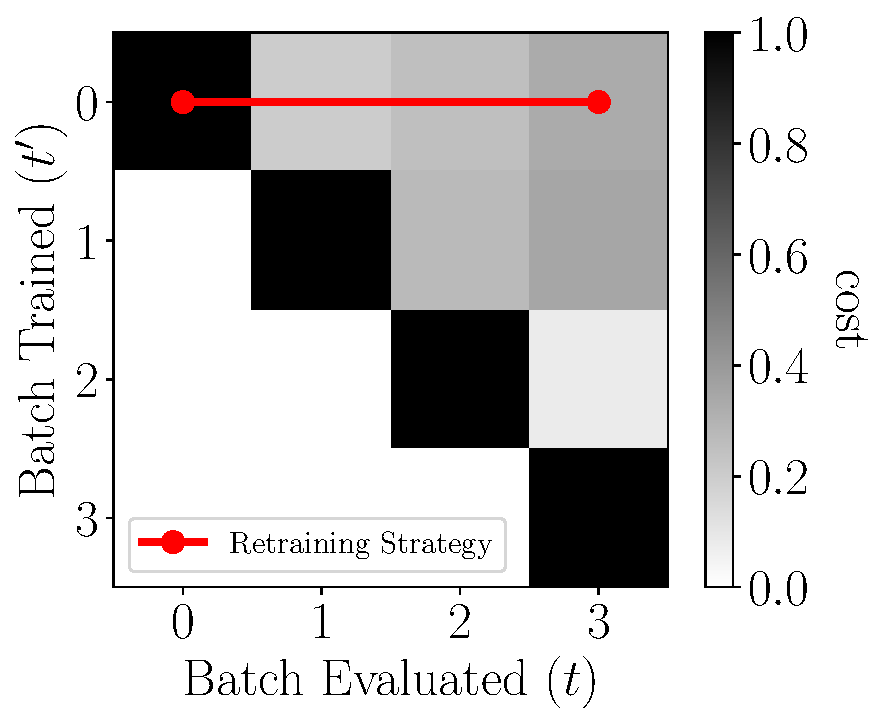
\includegraphics[width=0.7\textwidth]{figs/far_queries.pdf}
            \end{center}
          \end{minipage}%
          \begin{minipage}{0.5\textwidth}
            \begin{center}
            %   {\footnotesize Scenario 2}\\[1mm]
              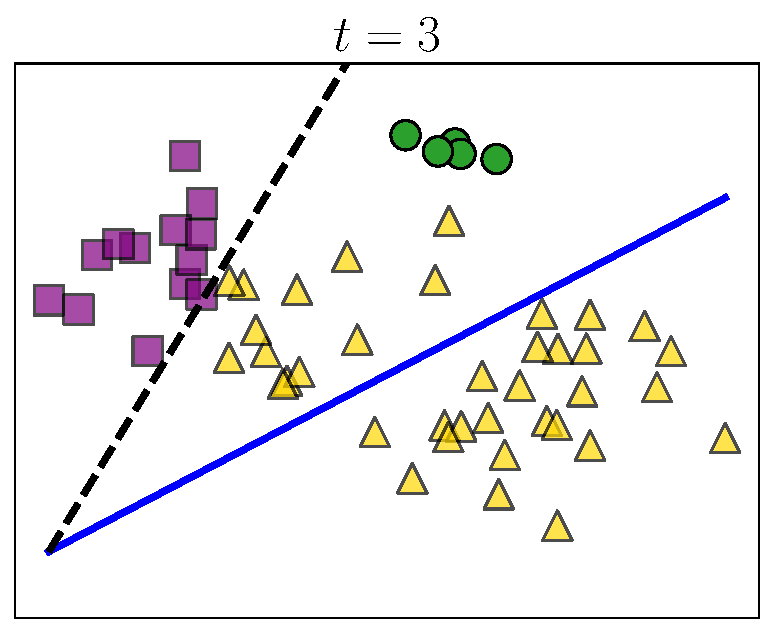
\includegraphics[width=0.7\textwidth]{figs/near_queries_illustration.pdf}\\[1mm]
              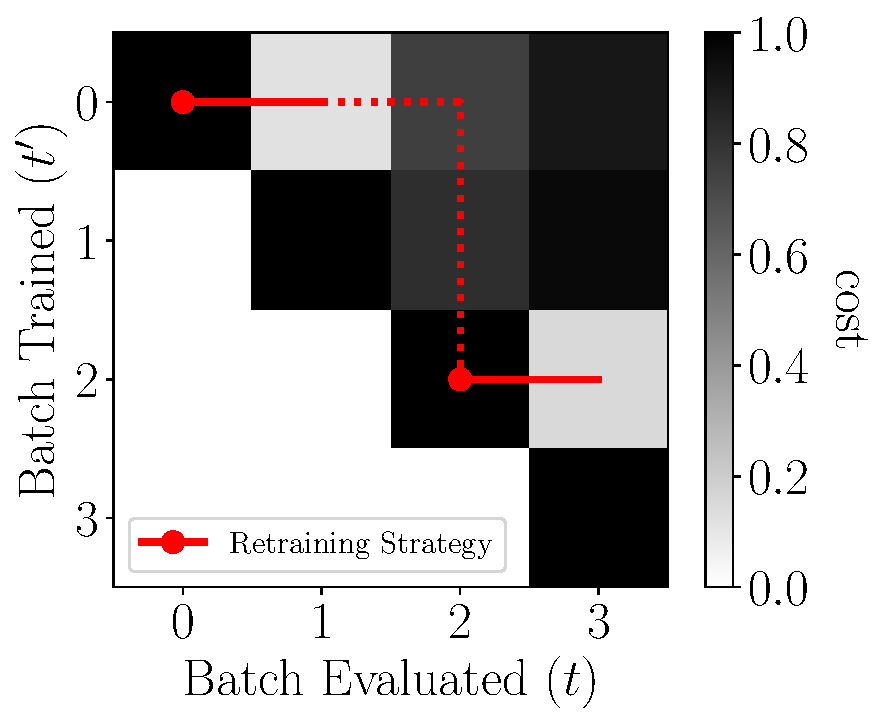
\includegraphics[width=0.7\textwidth]{figs/near_queries.pdf}
          \end{center}
        \end{minipage}%
    

\end{frame}
\begin{frame}
    \frametitle{Analyzing Historical Documents}
    Data:
    \begin{itemize}
        \item 250K books and 1M newspapers from the 17th and 18th century
        \item Tons of heterogeneous metadata
        \begin{itemize}
            \item Collections of books and articles
            \item Publisher details
            \item Author information
        \end{itemize}
        \item Multi-modal data  
        \begin{itemize}
            \item Scanned page images
            \item OCR text
            \item XML style structured page layouts
        \end{itemize}
    \end{itemize}
    Use cases:
    \begin{itemize}
        \item General data exploration
        \item Reception studies with Text Reuses   
        \item Top quotes of authors
    \end{itemize}
\end{frame}

\begin{frame}
    \frametitle{Reception Studies with Text Reuse}
    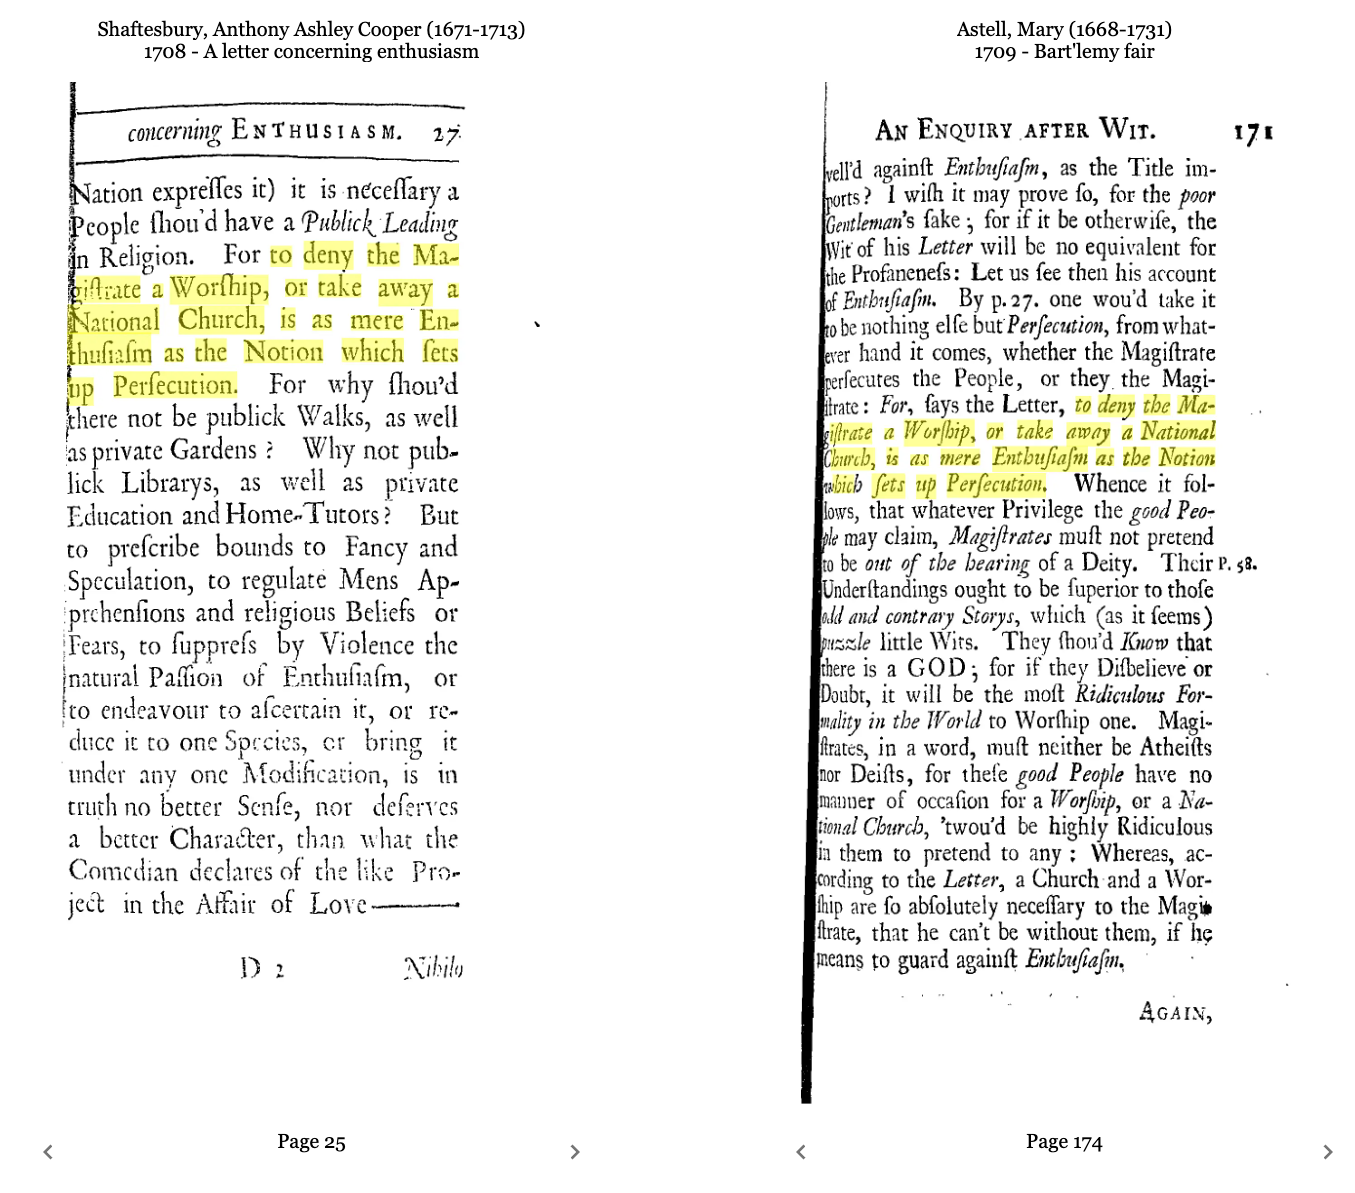
\includegraphics[width=\textwidth]{figs/Reception-Reader-Example.png}


\end{frame}

\begin{frame}[fragile]
    \frametitle{Identifying Text Reuse}


        However, OCR texts are very noisy
        \begin{block}{\centering Document 1 string}
            \footnotesize
            \begin{verbatim}
            to deny the Ma-
            tifl:ate a Worflip, or take away a
            hational Church, is as mere En-
            Ihufiafin as the Notion which sets
            uip Persecution    
            \end{verbatim}
        \end{block}    
        \begin{block}{\centering Document 2 string}
            \footnotesize
            \begin{verbatim}
            , to deny the Ala-
            inrate a ITorftip, or take awvay a National
            'uircb, is as mere Entnztfiafm as the Notion
            .bic fJets tup Persecution. W
            \end{verbatim}
        \end{block}    
        How to identify text reuses?
        \begin{itemize}
            \item Use BLAST to do fuzzy alignment
        \end{itemize}
\end{frame}

\begin{frame}[fragile]
    \frametitle{Pre-Processing Pipeline}
    \begin{figure}[htbp]
        \centering
        \scalebox{0.5}{
        \newcommand\file[2]{%
    \begin{scope}[xshift=#1cm,yshift=#2cm]
      \draw[gray,thick] (0,0) -- (0,1.5) -- (0.7,1.5) -- (0.7,1.1) -- (1,1.1) -- (1,0) -- cycle;
      \draw[gray,thick] (0.7,1.5) -- (1,1.1);
      \foreach \y in {0.2,0.3,...,1.1}{
         \draw[thick] (0.2,\y) -- (0.8,\y);
         }
      \foreach \y in {1.1,1.2,...,1.4}{
         \draw[thick] (0.2,\y) -- (0.65,\y);
         }
        %  \draw[thick] (0.2,0.8) -- (0.6,0.8);
        %  \draw[thick] (0.2,1) -- (0.6,1);
    \end{scope}
}

% https://tex.stackexchange.com/questions/126161/how-can-i-draw-a-tikz-element-multiple-times-against-a-shaded-background
% \pgfkeys{/tikz/.cd,
%    at/.initial={(0,0)},
%    at/.get=\coordpos,
%    at/.store in=\coordpos,   
%    my tree/.code={
%     \draw[gray] \coordpos -- +(0,1.2) -- +(0.7,1.2) -- +(0.7,0.8) -- +(1,0.8) -- +(1,0) -- cycle;
%     \draw[gray] +(0.7,1.2) -- +(1,0.8);
%     \foreach \y in {0.2,0.4,0.6}{
%         \draw (0.2,\y) -- (0.8,\y);
%         \draw (0.2,0.8) -- (0.6,0.8);
%         \draw (0.2,1) -- (0.6,1);
%     }
%    }
% }
\begin{tikzpicture}
    \tikzset{
      piece/.style 2 args={red,draw,thick,rectangle,anchor=south west,minimum width=#1,minimum height=#2},
      defrag piece/.style 2 args={blue,draw,thick,rectangle,anchor=south west,minimum width=#1,minimum height=#2},
      source piece/.style 2 args={orange,draw,very thick,rectangle,anchor=south west,minimum width=#1,minimum height=#2},
      destination piece/.style 2 args={green!50!black,draw,very thick,rectangle,anchor=south west,minimum width=#1,minimum height=#2},
      reuse/.style={red,-,very thick},
      defrag reuse/.style={blue,-,very thick},
      reception/.style={black,-{Latex[scale=1]},very thick},
      cluster/.style={violet,-,very thick,rounded corners=10pt,rectangle}
    }
    \begin{scope}[local bounding box=scope1]
    % \draw [help lines] (0,-2) grid (4,4);
    \file{0}{0}
    \node at (0.5,1.65) {A};
    \node[piece={0.8cm}{0.4cm}] at (0.1,0.1) (tr11) {};
    \node[piece={0.54cm}{0.4cm}] at (0.1,1.1) (tr12) {};
    \file{1.5}{1.5}
    \node at (2,3.15) {B};
    \node[piece={0.8cm}{0.4cm}] at (1.55,1.55) (tr21) {};
    \node[piece={0.78cm}{0.5cm}] at (1.64,1.63) (tr22) {};
    \file{3}{0}
    \node at (3.5,1.65) {C};
    \node[piece={0.54cm}{0.4cm}] at (3.1,0.95) (tr31) {};
    \node[piece={0.8cm}{0.4cm}] at (3.1,0.1) (tr32) {};
    \file{1.5}{-1.5}
    \node at (2,0.15) {D};
    \node[piece={0.8cm}{0.4cm}] at (1.55,-1.45) (tr41) {};
    \node[piece={0.78cm}{0.5cm}] at (1.63,-1.36) (tr42) {};
    \draw[reuse] (tr12.east) -- (tr21.west);
    \draw[reuse] (tr11.east) -- (tr41.west);
    \draw[reuse] (tr42.east) -- (tr32.west);
    \draw[reuse] (tr22.east) -- (tr31.west);
    % \node at (2,-1.68) {};
    % \matrix [below left] at (current bounding box.north east) {
    % \node [piece={0.5cm}{0.1cm},label=right:Piece] {};\\
    % \node[reuse,inner sep=0,minimum width=4mm,draw,anchor= south west,label=right:Text Reuse] at ++(1mm,0) {};\\
    % };
    \end{scope}

    \begin{scope}[local bounding box=scope2,shift={(scope1.base east)},xshift=3cm]
    % \draw [help lines] (0,-2) grid (4,4);
    \file{0}{0}
    \node at (0.5,1.65) {A};
    \node[defrag piece={0.8cm}{0.4cm}] at (0.1,0.1) (tr11) {};
    \node[defrag piece={0.54cm}{0.4cm}] at (0.1,1.1) (tr12) {};
    \file{1.5}{1.5}
    \node at (2,3.15) {B};
    \node[defrag piece={0.8cm}{0.54cm}] at (1.58,1.6) (tr21) {};
    \file{3}{0}
    \node at (3.5,1.65) {C};
    \node[defrag piece={0.54cm}{0.4cm}] at (3.1,0.95) (tr31) {};
    \node[defrag piece={0.8cm}{0.4cm}] at (3.1,0.1) (tr32) {};
    \file{1.5}{-1.5}
    \node at (2,0.15) {D};
    \node[defrag piece={0.8cm}{0.54cm}] at (1.6,-1.4) (tr41) {};
    \draw[defrag reuse] (tr12.east) -- (tr21.west);
    \draw[defrag reuse] (tr11.east) -- (tr41.west);
    \draw[defrag reuse] (tr41.east) -- (tr32.west);
    \draw[defrag reuse] (tr21.east) -- (tr31.west);
    
    \draw[cluster] (-0.1,0.9) rectangle (4,2.3) ;
    \draw[cluster] (-0.1,0.6) rectangle (4.2,-1.5) ;
    % \draw[cluster] plot [smooth cycle] coordinates{(0.1,1) (3.8,0.95) (3.5,2) (2,2.25) (0.6,2) };
    % \draw[cluster] plot [smooth cycle] coordinates{(0.0,0.6)  (4,0.6) (3.5,-1) (2,-1.75) (0.55,-1)};
    \end{scope}

    \begin{scope}[local bounding box=scope3,shift={(scope2.base east)},xshift=3cm]
      % \draw [help lines] (0,-2) grid (4,4);
      \file{0}{0}
      \node at (0.5,1.65) {A};
      \node[source piece={0.8cm}{0.4cm}] at (0.1,0.1) (tr11) {};
      \node[destination piece={0.54cm}{0.4cm}] at (0.1,1.1) (tr12) {};
      \file{1.5}{1.5}
      \node at (2,3.15) {B};
      \node[source piece={0.8cm}{0.54cm}] at (1.58,1.6) (tr21) {};
      \file{3}{0}
      \node at (3.5,1.65) {C};
      \node[destination piece={0.54cm}{0.4cm}] at (3.1,0.95) (tr31) {};
      \node[destination piece={0.8cm}{0.4cm}] at (3.1,0.1) (tr32) {};
      \file{1.5}{-1.5}
      \node at (2,0.15) {D};
      \node[destination piece={0.8cm}{0.54cm}] at (1.6,-1.4) (tr41) {};
      \draw[reception] (tr11.east) -- (tr41.west);
      \draw[reception] (tr11.east) -- (tr32.west);

      \draw[reception] (tr21.west) -- (tr12.east);
      \draw[reception] (tr21.east) -- (tr31.west);
        
      \draw[cluster] (-0.1,0.9) rectangle (4,2.3) ;
      \draw[cluster] (-0.1,0.6) rectangle (4.2,-1.5) ;
    %   \draw[cluster] plot [smooth cycle] coordinates{(0.1,1) (3.8,0.95) (3.5,2) (2,2.25) (0.6,2) };
    %   \draw[cluster] plot [smooth cycle] coordinates{(0.0,0.6)  (4,0.6) (3.5,-1) (2,-1.75) (0.55,-1)};
      \end{scope}

      \draw [->,black,very thick] ($(scope1.east)!0.1!(scope2.west)$) -- ($(scope1.east)!0.9!(scope2.west)$)  node[midway,above]{Defragment} node[midway,below] {\& Cluster};
      \draw [->,black,very thick] ($(scope2.east)!0.1!(scope3.west)$) -- ($(scope2.east)!0.9!(scope3.west)$)  node[midway,above]{Identify Sources} node[midway,below] {\& Destinations};

    \matrix [draw,matrix anchor = south,yshift=5mm] at ($(scope1.north west)!0.5!(scope3.north east)$) {
    \node [inner sep=0,label=right:Doc,anchor=south west] at (0,-0.5mm){\faFileTextO}; & 
    \node [piece={0.5cm}{0.1cm},label=right:Piece] {}; & 
    \node[reuse,inner sep=0,minimum width=4mm,draw,anchor=south west,label=right:Text Reuse] at ++(0,1mm) {}; & 
    \node [defrag piece={0.5cm}{0.1cm},label=right:Defrag Piece] {}; & 
    \node[defrag reuse,inner sep=0,minimum width=4mm,draw,anchor= south west,label=right:Defrag Text Reuse] at ++(0,1mm) {}; & 
    \node[draw,cluster,anchor=south west,minimum width=0.5cm,minimum height=0.1cm,rounded corners=2pt,rectangle,label=right:Cluster] {};& 
    \node [source piece={0.5cm}{0.1cm},label=right:Source Piece] {}; & 
    \node [destination piece={0.5cm}{0.1cm},label=right:Destination Piece] {}; & 
    \draw[reception] (0,1mm) -- (5mm,1mm) node[inner sep =0,minimum size =0,right,anchor=west] {Reception};
    \\
    };
\end{tikzpicture}

%

% \node[label=below:Document,inner sep=0,minimum size =0] {\faFileTextO}; & 
% \node [piece={0.5cm}{0.3cm},anchor=center,label=below:Piece] {}; & 
% \draw[reuse] (0,0mm) -- (5mm,0mm) node[inner sep =0,minimum size =0,midway,below=4mm,anchor=center,black] {Text Reuse};&
% \node [defrag piece={0.5cm}{0.3cm},anchor=center,label=below:Defrag Piece] {};& 
% \draw[defrag reuse] (0,0mm) -- (5mm,0mm) node[inner sep =0,minimum size =0,midway,below=4mm,anchor=center,black] {Defrag Text Reuse};&
% \draw[cluster] (0,0mm) -- +(5mm,0mm) node[inner sep =0,minimum size =0,midway,below=3.6mm,anchor=center,black] {~Cluster};&
% \node [source piece={0.5cm}{0.3cm},anchor=center,label=below:Source Piece] {}; & 
% \node [destination piece={0.5cm}{0.3cm},anchor=center,label=below:Destination Piece] {}; & 
% \draw[reception] (0,0mm) -- +(5mm,0mm) node[inner sep =0,minimum size =0,midway,below=4mm,anchor=center] {Reception};
% \\
        }
        \caption{Illustration of the pre-processing pipeline for text reuses. The hits from BLAST (red) are first defragmented (blue) and then clustered (purple). Then in each cluster, the piece from the earliest document is identified as the source (yellow) and the rest are destinations (green). The directed edge between a source and destination piece is a reception edge.}
    \end{figure}
\end{frame}

\begin{frame}
    \frametitle{ETL Pipeline Implementation}
    \only<1>{
    \begin{itemize}
        \item Starts with {\bf 6.31 billion} pairs of reuses from BLAST
        \item ETL implemented in Apache Spark 
        \item Uses Dagster for asset management
        \item Loads processed data into MariaDB for downstream queries
        \item Tables used for front-end user queries 
    \end{itemize}
    }
    \only<2>{
    \includegraphics<2>[width=\textwidth]{figs/ERD.pdf}}
    

\end{frame}

\begin{frame}
    \frametitle{Related Publications}

    \begin{enumerate}
        \item Paper IV: \citet{Rosson-2023}
        \begin{itemize}
            \item \emph{Reception reader: Exploring text reuse in early modern british publications}
            \item Front-end user interface for browsing reuses
        \end{itemize}
        \item Paper V: \citet{des6}
        \begin{itemize}
            \item \emph{A Comparative text similarity analysis of the works of Bernard Mandeville}
            \item Study using the data and interfaces from Paper IV
        \end{itemize}
        \item Paper VI: \citet{mahadevan2024optimizing}
        \begin{itemize}
            \item \emph{Optimizing a Data Science System for Text Reuse Analysis}
            \item Studies design choices to optimize performance of the system
            \item Plans to scale interface from Paper IV based on insights
        \end{itemize}
    \end{enumerate}


\end{frame}
\begin{frame}
    \frametitle{Scalability and Robustness}
    \begin{itemize}
        \item Paper II: \citet{merchant2022JANE}
        \begin{itemize}
            \item Scaled up GNN alternative from \citet{merchant2022JANEorig} to run effectively on graphs with millions of nodes
        \end{itemize}
        \item Paper III: \citet{10.1145/3511808.3557687}
        \begin{itemize}
            \item Explored the robustness of Sketched Linear Networks from \citet{tai2018sketch} to adversarial attacks
        \end{itemize}
        \item Paper VIII?: 
        \begin{itemize}
            \item Original algorithm from \citet{wang2023fmmd}
            \item Re-implemented for edge-case requirement in Historical Project
            \item Nearly $200\times$ speed-up compared to original code
            \item Plans to develop theory and code for distributed algorithm 
        \end{itemize}
    \end{itemize}
\end{frame}

\begin{frame}
    \frametitle{Next Steps}
    \begin{enumerate}
        \item Complete a few more transferrable skill credits
        \item Start Writing Thesis
        \item Work on Paper VIII in tandem 
    \end{enumerate}
    

\end{frame}

\begin{frame}[allowframebreaks]
    \frametitle{References}
    \bibliographystyle{plainnat}
    \bibliography{references.bib}
  \end{frame}

\end{document}